\chapter{AI Data Assimilation}


%==============================================================================
%
%==============================================================================
\section{Introduction to AI-based Data Assimilation}

In the rapidly advancing field of Numerical Weather Prediction (NWP), the integration of observational data into numerical models is fundamental to achieving high-quality forecast accuracy. This process, known as \textit{data assimilation}, combines observed data with model outputs to improve initial conditions and refine forecast predictions. Data assimilation techniques have evolved significantly over the years, with traditional methods such as \textit{variational data assimilation (3D-Var)}, \textit{ensemble Kalman filters (EnKF)}, and \textit{particle filters} serving as the backbone of current NWP systems. These methods rely heavily on computational models to assimilate data and refine predictions, ensuring that weather forecasting remains reliable and precise.

Today, in the time of AI, we have two approaches to using observations. One approach is the direct integration of observations into the neural networks for forecasting, i.e. observations are used either additional or as only input for calculating a forecast based on neural network architectures. The second approach is to use observations to calculate an analysis minimizing a functional with a particular loss function motivated from Bayesian arguments. This reflects a traditional data assimilation approach, but now carried out with AI/ML based neural architectures. The AI-Var of Keller and Potthast is one of these algorithms, compare \url{https://arxiv.org/abs/2406.00390}. 

\begin{figure}[ht]
\centering
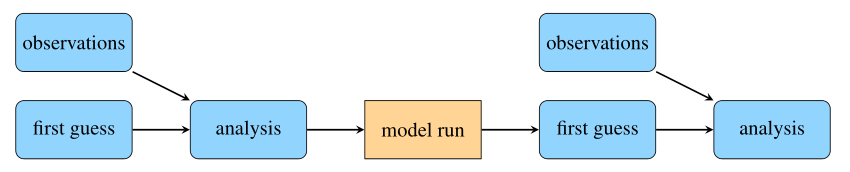
\includegraphics[width=0.7\textwidth]{images/aivar3.png}
\caption{Classical data assimilation cycle, where observations and the first guess are integrated to generate an analysis. The cycle continues with model runs and updates based on new observations.}
\end{figure}


%------------------------------------------------------------------------------
%
%------------------------------------------------------------------------------
\subsection{AI-Based Methods for Data Assimilation}

The emergence of AI, particularly deep learning, presents an exciting opportunity to enhance the capabilities of NWP systems. AI-based models have shown the potential to emulate complex physical calculations traditionally handled by numerical models. Notably, AI can dramatically reduce computational costs, thereby speeding up data assimilation and forecasting processes. The primary advantage of AI in NWP is its ability to learn complex relationships from large datasets, allowing for faster and more flexible predictions.

The main objective of using AI in NWP is to create more efficient models that can predict weather outcomes with minimal computational overhead. This is for example accomplished by training deep learning models to replicate the processes typically used in traditional numerical models, such as simulating atmospheric dynamics, computing forecast scenarios, and applying corrections through assimilation.

%------------------------------------------------------------------------------
%
%------------------------------------------------------------------------------
\subsection{AI-based Variational Data Assimilation (AI-Var)}

In this tutorial, we introduce the concept of \textit{AI-based variational data assimilation} (AI-Var), a novel approach that aims to replace traditional data assimilation techniques with AI-driven models. Unlike hybrid methods that combine machine learning with classical approaches, AI-Var fully integrates the data assimilation process into a neural network. The neural network is trained to minimize a cost function that mirrors the variational assimilation framework.

\begin{figure}[ht]
\centering
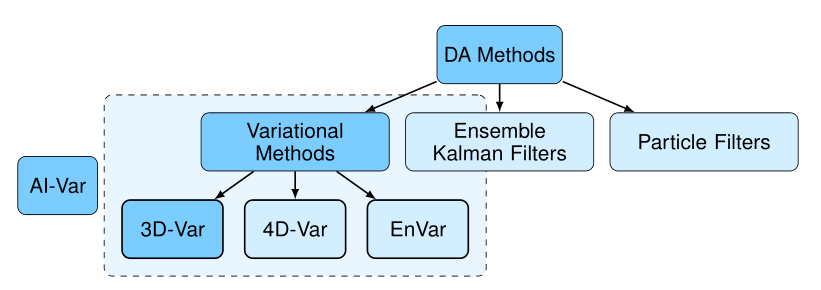
\includegraphics[width=0.7\textwidth]{images/aivar2.png}
\caption{The AI-Var method within the broader context of data assimilation methods. AI-Var is a part of variational methods, which include 3D-Var, 4D-Var, and EnVar, all of which belong to the family of Data Assimilation (DA) methods.}
\end{figure}

The standard variational data assimilation process (such as 3D-Var) seeks to minimize the following cost function:

\[
J(\mathbf{x}) = \frac{1}{2} (\mathbf{x} - \mathbf{x}_b)^T \mathbf{B}^{-1} (\mathbf{x} - \mathbf{x}_b) + \frac{1}{2} (\mathbf{y} - \mathbf{H}(\mathbf{x}))^T \mathbf{R}^{-1} (\mathbf{y} - \mathbf{H}(\mathbf{x}))
\]

In this cost function:
- \( \mathbf{x}_b \) is the background state (first guess),
- \( \mathbf{y} \) are the observations,
- \( \mathbf{B} \) is the background error covariance matrix,
- \( \mathbf{R} \) is the observation error covariance matrix,
- \( \mathbf{H}(\mathbf{x}) \) is the observation operator, which maps the model state to the observation space.

The neural network is trained to minimize this cost function, but without relying on pre-existing analysis datasets. Instead, it learns the mapping from input data (observations and first guess) directly to the analysis, making it a fully data-driven system.

%------------------------------------------------------------------------------
%
%------------------------------------------------------------------------------
\subsection{Conceptual Framework for AI-Var}

The AI-Var method integrates the data assimilation process into the structure of a neural network. Rather than relying on classical analysis methods, AI-Var learns to predict the analysis directly from the input data.


The approach can be illustrated conceptually as follows:

\begin{figure}[ht]
\centering
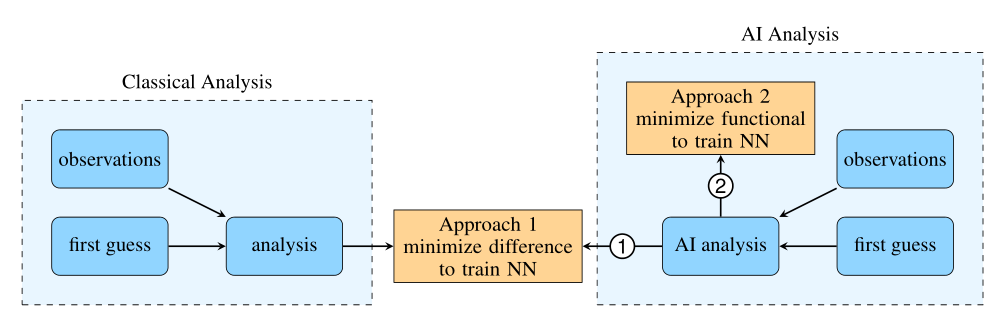
\includegraphics[width=0.7\textwidth]{images/aivar1.png}
\caption{Conceptual framework for AI-based data assimilation, where the classical data assimilation process is replaced by a neural network that learns the analysis directly from the observations and first guess.}
\end{figure}

In this figure, the input data consists of the first guess (\( \mathbf{x}_b \)) and the observations (\( \mathbf{y} \)). Further, the neural network learns the functional relationship between these inputs and the desired analysis (\( \mathbf{x}_a \)). The neural network is trained to minimize the variational cost function, ensuring that the analysis \( \mathbf{x}_a \) is as close as possible to the optimal state based on the observations. The analysis $x_{a}$ is not needed for this training process, such that we can retrain without calculating reanalysis fields beforehand. 

%=\*80
% AI-Var Training and Loss Function
%=\*80

%------------------------------------------------------------------------------
%
%------------------------------------------------------------------------------
\subsection{AI-Var Training and Loss Function}

The key to AI-Var is training a neural network to minimize the cost function defined earlier. The cost function can be directly used as the loss function for training the model. Instead of training on the predefined analysis states, the neural network learns to minimize the difference between the background state and the observations, incorporating the error covariances directly into the training process.

The loss function in AI-Var becomes:

\[
L = (\hat{\mathbf{x}} - \mathbf{x}_b)^T \mathbf{B}^{-1} (\hat{\mathbf{x}} - \mathbf{x}_b) + (\hat{\mathbf{y}} - \mathbf{y})^T \mathbf{R}^{-1} (\hat{\mathbf{y}} - \mathbf{y})
\]

where: \( \hat{\mathbf{x}} \) is the output of the neural network (the predicted analysis), and \( \hat{\mathbf{y}} = \mathbf{H}(\hat{\mathbf{x}}) \) is the model equivalent of the predicted analysis.

This formulation allows for the direct integration of the data assimilation process into a deep learning framework, providing a computationally efficient and flexible alternative to traditional methods.


In conclusion, the AI-Var approach presents a promising alternative to traditional data assimilation techniques. By integrating the data assimilation process into a neural network, AI-Var can potentially improve computational efficiency and accuracy in weather forecasting. The initial results from both idealized and real-world test cases demonstrate the feasibility of replacing classical data assimilation systems with AI-driven models. Future work will focus on further refining the AI-Var method, including the use of more advanced neural network architectures and exploring the application of AI in high-dimensional, real-world weather prediction scenarios.


%==============================================================================
%
%==============================================================================
\section{Training for AI-based Data Assimilation (AIDA)}

In this section, we will walk through the steps involved in training a simple machine learning model using the AIDA code, a framework for AI-based data assimilation (AI-Var). This tutorial introduces the various modules and functionalities required to set up and train the model.

%=\*80
% Setting up the Environment and Data Paths
%=\*80

%------------------------------------------------------------------------------
%
%------------------------------------------------------------------------------
\subsection{Setting up the Environment and Data Paths}

First, we need to import the necessary modules and set up the environment for our calculations. We will use PyTorch, a popular machine learning library, to train the neural network. Additionally, we check if a GPU is available for faster computations.

\begin{codeonly}{Imports, Device Setup}
import torch
import matplotlib.pyplot as plt

device = "cuda" if torch.cuda.is_available() else "cpu"
print(f"Set device to {device}.")
\end{codeonly}

Here, the `torch` module is imported for neural network computations, and `matplotlib.pyplot` is used for plotting. The device is set to GPU if available, otherwise, it defaults to the CPU.

Next, we define the paths to the data files required for training. These include paths to grid files, observation data, and forecast data.

\begin{codeonly}{Paths Setup}
grid_file = '/hpc/uwork/fe11bacy/invar_new/invar_0027_R03B08_L120_20231113_tiles.grb'
fg_path = '/hpc/uwork/tdeppisc/AIDA_data/ICON-EU'
synop_path = '/hpc/uwork/tdeppisc/AIDA_data/SYNOP'
output_path = 'showcase_output'
\end{codeonly}

The grid file contains the necessary static data for the model, such as the geographical grid of the simulation. The forecast (`fg\_path`) and observation (`synop\_path`) paths hold the simulation results and observational data, respectively.

%------------------------------------------------------------------------------
%
%------------------------------------------------------------------------------
\subsection{Defining Time Interval and Domain Boundaries}

For training, we define a time interval and the domain boundaries over which we will perform the data assimilation. Here, we use a `TimeSeries` class to define the training time period from May 10, 2023, to May 10, 2023, at 3-hour intervals.

\begin{codeonly}{Time Series, Domain Boundaries}
from util import TimeSeries
valid_times = TimeSeries(start='20230510000000', end='20230510230000', step={'hours':3})
print(valid_times)
\end{codeonly}

We also set the geographical domain for our observations by specifying the latitude and longitude bounds.

\begin{codeonly}{Geo Domain}
domain = {'lon_min': 7.5, 'lon_max': 8.5, 'lat_min': 49.5, 'lat_max': 50.5}
\end{codeonly}

This domain will restrict the data assimilation to the region of central Europe, specifically around the ICON-EU model grid.

%------------------------------------------------------------------------------
%
%------------------------------------------------------------------------------
\subsection{Loading Observation Data}

We load the observation data using the `ObservationDataset` class, which is a container for observations at different times. The dataset is populated with observational data from the SYNOP files.

\begin{codeonly}{Load Observation Data}
from observations import ObservationDataset
obs = ObservationDataset(valid_times=valid_times, domain=domain)
\end{codeonly}

Once the `ObservationDataset` is initialized, we add the observational data from the SYNOP files and associate the relevant metadata, including observation errors and variable descriptions.

\begin{codeonly}{Add Feedback Data}
obs.add_feedback_data(path=synop_path, obs_type='SYNOP', fdbk_type='mon', model='ICON-EU', n_obs=50, observation_descriptions=[{"varno": 39, "obs_err": 1.0}])
\end{codeonly}

Here, we specify the observation type (`SYNOP`), model (`ICON-EU`), and the error associated with the temperature observations.

To verify the data, we can print an overview of the dataset:

\begin{codeonly}{Verify Data}
print(obs)
\end{codeonly}

The data structure is hierarchical, with each time step containing observation types, such as `SYNOP`, each with its corresponding data.

%------------------------------------------------------------------------------
%
%------------------------------------------------------------------------------
\subsection{Visualizing the Observation Data}

After loading the observation data, we can access and visualize it. For example, we can extract the temperature observations at a specific time step and plot them on a map.

\begin{codeonly}{Visualize Observations}
foo = obs.time_steps['20230510120000'].obs_types["SYNOP"]
plt.scatter(foo.get_column('lon'), foo.get_column('lat'), c=foo.get_column('obs'), vmin=284., vmax=290., marker='s', edgecolor='k')
plt.colorbar()
\end{codeonly}

This plot shows the SYNOP observations as a scatter plot with temperature values represented by color.

%------------------------------------------------------------------------------
%
%------------------------------------------------------------------------------
\subsection{Loading Forecast Data}

Similarly, we load forecast data using the `ForecastDataset` class, which contains the forecast data for each time step. We define the forecast grid and add fields from the ICON-EU model.

\begin{codeonly}{Load Forecast Data}
from forecasts import ForecastDataset
fg = ForecastDataset(valid_times=valid_times)

static_fields = {'CLON':0, 'CLAT':0}
fg.add_analysis_grid(grid_file=grid_file, model="ICON-EU", static_field_descriptions=static_fields, domain=domain, grid_3d=False)
print(fg.analysis_grid)
\end{codeonly}

Next, we add the first guess fields from the ICON DREAM reanalysis.

\begin{codeonly}{Add Forecast Fields}
fg_fields = {'T_2M':2}
fg.add_ICON_fg(model="ICON-EU", layer_descriptions=fg_fields, path=fg_path, use_index_file=False)
print(fg)
\end{codeonly}

The `ForecastDataset` class allows us to work with model output data and prepares it for integration into the data assimilation process.

%------------------------------------------------------------------------------
%
%------------------------------------------------------------------------------
\subsection{Combining Observation and Forecast Data}

For the data assimilation process, we need to combine both the observation data and the forecast data into a single dataset. We do this by creating a `DADataset` object.

\begin{codeonly}{Combine Data}
from datasets import DADataset
training_dataset = DADataset(obs, fg)
\end{codeonly}

This dataset can be split into training and validation sets. Here, we use 10\% of the data for validation.

\begin{codeonly}{Validation Split}
validation_dataset = training_dataset.create_validation_dataset(random_fraction=0.1)
training_dataset.check_completeness(if_incomplete="deleteData")
validation_dataset.check_completeness(if_incomplete="deleteData")
\end{codeonly}

%------------------------------------------------------------------------------
%
%------------------------------------------------------------------------------
\subsection{Defining the Data Assimilation Model}

Now we define the machine learning model. For simplicity, we use an encoder-decoder architecture. The encoder processes both the forecast data and the observation data, while the decoder reconstructs the analysis.

\begin{codeonly}{Model Definition}
from models import DAAutoencoder, InSituFO
model = DAAutoencoder(n_target=1, n_latent=256, forward_operators={"SYNOP": InSituFO()}, activation=torch.nn.PReLU(), batch=training_dataset.test_batch)
print(model)
\end{codeonly}

This model is initialized with certain parameters, such as the number of latent variables, the forward operators, and activation functions.

%=\*80
% Loss Function and Optimization
%=\*80

\subsection{Defining the Loss Function}

The loss function is based on the data assimilation functional, which is used to optimize the model. It combines the background state and the observations in a cost function.

\begin{codeonly}{Loss Function Definition}
from losses import DALoss, GaussianBMatrix, DiagonalRMatrix
loss_function = DALoss(alpha=0.1, b_matrix=GaussianBMatrix(grid_information=fg.analysis_grid, sigma_horz=20., eps=0.01), r_matrices={"SYNOP": DiagonalRMatrix(n_obs=50)})
print(loss_function)
\end{codeonly}

This loss function defines the balance between the forecast and observation data.


\begin{figure}[ht]
\centering
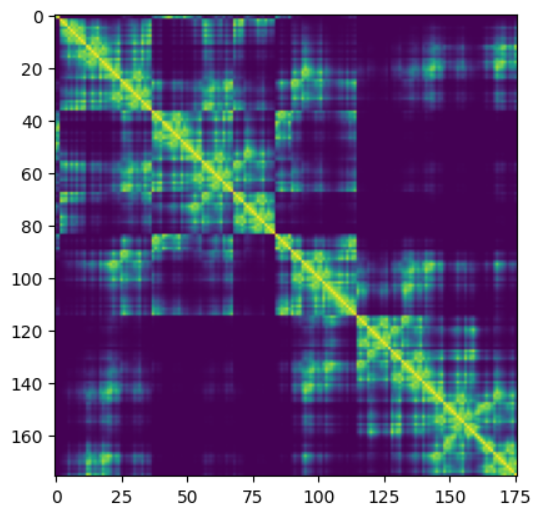
\includegraphics[width=0.7\textwidth]{images/aivar_B_matrix.png}
\caption{AI-Var B Matrix, showing the structure of the background error covariance matrix used in the variational data assimilation process. The matrix reveals the spatial correlations between the forecast errors at different grid points.}
\end{figure}

%------------------------------------------------------------------------------
%
%------------------------------------------------------------------------------
\subsection{Training the Model}

We use the `DATrainer` class to handle the training process. The model is trained for 100 epochs with the Adam optimizer.

\begin{codeonly}{Training}
from training import DATrainer
trainer = DATrainer(training_dataset=training_dataset, validation_dataset=validation_dataset, model=model, loss_function=loss_function, optimizer=torch.optim.Adam(model.parameters(), lr=0.0001), device=device, batch_size=8, output_path=output_path)
trainer.train_model(n_epochs=100)
trainer.print_summary()
\end{codeonly}

The training process updates the model parameters based on the loss function and training data.

\begin{figure}[ht]
\centering
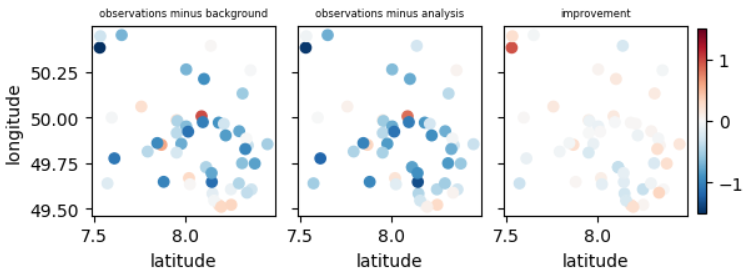
\includegraphics[width=0.7\textwidth]{images/aivar_o-b_o-a.png}
\caption{Comparison of observations minus background (o-b) and observations minus analysis (o-a). The plot on the left shows the difference between the observations and the forecast background, while the plot on the right shows the difference after the analysis. The middle plot highlights the improvements made during the assimilation process.}
\end{figure}

%------------------------------------------------------------------------------
%
%------------------------------------------------------------------------------
\subsection{Conclusion and Saving the Model}

After training the model, we save it for future use. The trained model can then be applied to new data to make predictions.

\begin{codeonly}{Save Model}
filename = "my_ai_model.pt"
torch.save(model, filename)
\end{codeonly}

We can now load this saved model to make predictions or continue training.


%==============================================================================
%
%==============================================================================
\section{Inference for AI-based Data Assimilation}

After training an AI model for data assimilation, the next crucial step is applying the model to new, unseen data. In this section, we will guide you through the process of using a pretrained AI model to perform inference on a larger dataset. The model is applied to a month's worth of data, and we demonstrate how to load the model, apply it to observations and forecasts, and visualize the results.

%------------------------------------------------------------------------------
%
%------------------------------------------------------------------------------
\subsection{Initial Configuration}

Before performing inference, we need to set up the environment. This includes importing the necessary libraries, setting the computation device (CPU or GPU), and defining the paths to the required data files.

\begin{codeonly}{Imports, Device Setup}
import torch
import matplotlib.pyplot as plt
import numpy as np

device = "cuda" if torch.cuda.is_available() else "cpu"
print(f"Set device to {device}.")
\end{codeonly}

The model will be executed on a GPU if available, which accelerates computations.

Next, we define the paths to the required files: grid files, forecast data, and observation data.

\begin{codeonly}{Paths Setup}
grid_file = '/hpc/uwork/fe11bacy/invar_new/invar_0027_R03B08_L120_20231113_tiles.grb'
fg_path = '/hpc/uwork/tdeppisc/AIDA_data/ICON-EU'
synop_path = '/hpc/uwork/tdeppisc/AIDA_data/SYNOP'
output_path = 'showcase_output'
\end{codeonly}

These paths point to the data used in the inference process.

%------------------------------------------------------------------------------
%
%------------------------------------------------------------------------------
\subsection{Loading a Pre-trained Model}

Once the environment is set up, we load a pre-trained model for inference. The model was trained using a graph neural network architecture, and we can now apply it to the new dataset.

\begin{codeonly}{Model Loading}
filename = "/hpc/uwork/tdeppisc/AIDA_data/models/gnn_example.pt"
model = torch.load(filename, map_location=torch.device(device), weights_only=False)
print(model)
\end{codeonly}

The model is loaded from a specified file and ready for inference.

%------------------------------------------------------------------------------
%
%------------------------------------------------------------------------------
\subsection{Loading Data}

The data loading process for inference is similar to that used during training. We load both the observational data and forecast data for the inference period, which spans a full month.

\begin{codeonly}{Observation Data Loading}
from observations import ObservationDataset

obs = ObservationDataset(valid_times=valid_times, domain=domain)
obs.add_feedback_data(path=synop_path, obs_type='SYNOP', fdbk_type='mon', model='ICON-EU', n_obs=50, observation_descriptions=[{"varno": 39, "obs_err": .5}])
print(obs)
\end{codeonly}

Here, the `ObservationDataset` class is used to load observational data for the specified period and domain.

Similarly, the forecast data is loaded using the `ForecastDataset` class.

\begin{codeonly}{Forecast Data Loading}
from forecasts import ForecastDataset
fg = ForecastDataset(valid_times=valid_times)
fg.add_analysis_grid(grid_file=grid_file, model="ICON-EU", static_field_descriptions={'CLON':0, 'CLAT':0}, domain=domain, grid_3d=False, interpolation_method='inv_distances')
fg.add_ICON_fg(model="ICON-EU", layer_descriptions={'T_2M':2}, path=fg_path, use_index_file=True)
print(fg)
\end{codeonly}

Now we have both the observational and forecast datasets ready to be used for inference.

%------------------------------------------------------------------------------
%
%------------------------------------------------------------------------------
\subsection{Applying the Model to Data}

With the model and data in place, we can proceed to apply the model to the dataset. The `DAInference` class is used for this purpose.

\begin{codeonly}{Applying Model to Data}
from inference import DAInference
inference = DAInference(model, dataset)
\end{codeonly}

This class provides convenient methods to extract and process the data after applying the model.

For example, to retrieve the observations, first guess in observation space, and the analysis, we can use the following commands:

\begin{codeonly}{Retrieve Data}
print('observations:')
print(inference.get_obs_data('obs','20230115120000','SYNOP'))

print('\nfirst guess in observation space')
print(inference.get_obs_data('h_fg','20230115120000','SYNOP'))

print('\nanalysis in observation space with coordinates')
print(inference.get_obs_data('h_an','20230115120000','SYNOP', return_coordinates=True))
\end{codeonly}

These commands extract the data for a specific time step, providing insight into the analysis and the first guess in the context of observations.

%------------------------------------------------------------------------------
%
%------------------------------------------------------------------------------
\subsection{Creating Statistics from Inference Results}

We can calculate various statistics to evaluate the model’s performance. For example, the `ObservationStatistics` class is used to calculate statistics such as the observation-minus-background (o-b) and observation-minus-analysis (o-a) for each time step.

\begin{codeonly}{Statistics Creation}
from obs_stats import ObservationStatistics
obs_stats = ObservationStatistics(inference)

my_stats = obs_stats.create_statistics([
        {"description": "2m temperature (o-b)", "obs_type": "SYNOP", "stat_type": "o-b", "stat_val" : "values", "filter": {"varno": 39}},
        {"description": "2m temperature (o-a)", "obs_type": "SYNOP", "stat_type": "o-a", "stat_val" : "values", "filter": {"varno": 39}}])
\end{codeonly}

We can further aggregate these statistics over time, for example, to calculate global averages.

\begin{codeonly}{Aggregating Statistics}
ob_total = my_stats[0].get_average('all')
oa_total = my_stats[1].get_average('all')

print("global statistics")
print(ob_total)
print(oa_total)
\end{codeonly}

These aggregated statistics provide a broader view of model performance over the entire inference period.


\begin{figure}[ht]
\centering
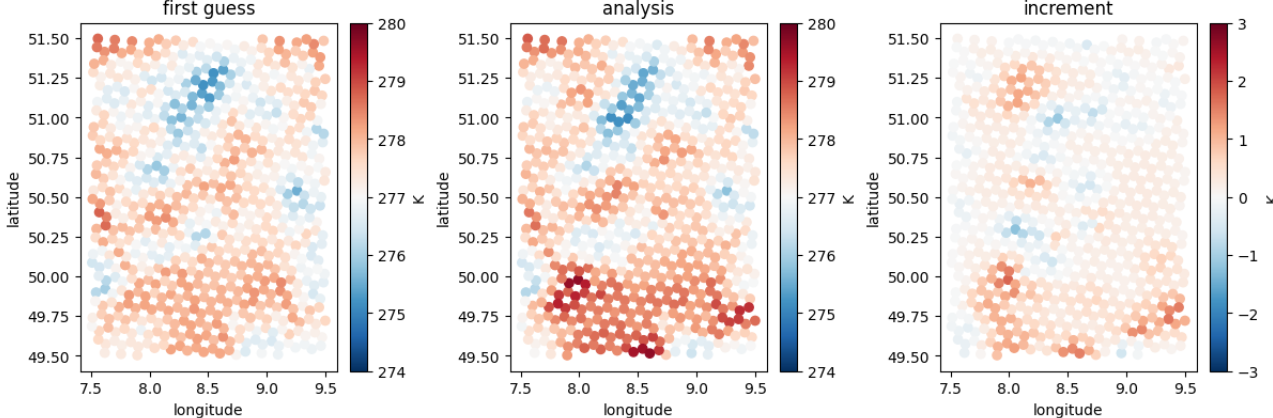
\includegraphics[width=\textwidth]{images/aivar4.png}
\caption{AI-Var results for the 2m temperature field. The left panel shows the first guess (forecast), the middle panel shows the resulting analysis, and the right panel shows the increment (analysis minus first guess). The spatial structure of corrections introduced by the neural network is clearly visible.}
\end{figure}
%------------------------------------------------------------------------------
%
%------------------------------------------------------------------------------
\subsection{Plotting Statistics and Results}

To visualize the results of the inference, we can plot various statistics such as bias, standard deviation, and the number of observations for each day.

\begin{codeonly}{Plotting Statistics}
fig, axs = plt.subplots(3,1, sharex=True, constrained_layout=True)

ob_daily = my_stats[0].get_average('years+months+days')
oa_daily = my_stats[1].get_average('years+months+days')

ax = axs[0]
ax.plot(ob_daily.mean, label="(o-b)")
ax.plot(oa_daily.mean, label="(o-a)")
ax.legend(loc='upper right')
ax.set_title('bias (2m temperature)')
ax.set_ylabel('K')

ax = axs[1]
ax.plot(ob_daily.std, label="(o-b)")
ax.plot(oa_daily.std, label="(o-a)")
ax.legend(loc='upper right')
ax.set_title('standard deviation (2m temperature)')
ax.set_ylabel('K')

ax = axs[2]
ax.plot(ob_daily.n_obs, label="(o-b)")
ax.plot(oa_daily.n_obs, label="(o-a)")
ax.legend(loc='upper right')
ax.set_title('number of observations')
ax.set_xlabel('days')
\end{codeonly}

This will generate three subplots showing the bias, standard deviation, and number of observations for each day in the period.

\begin{figure}[ht]
\centering
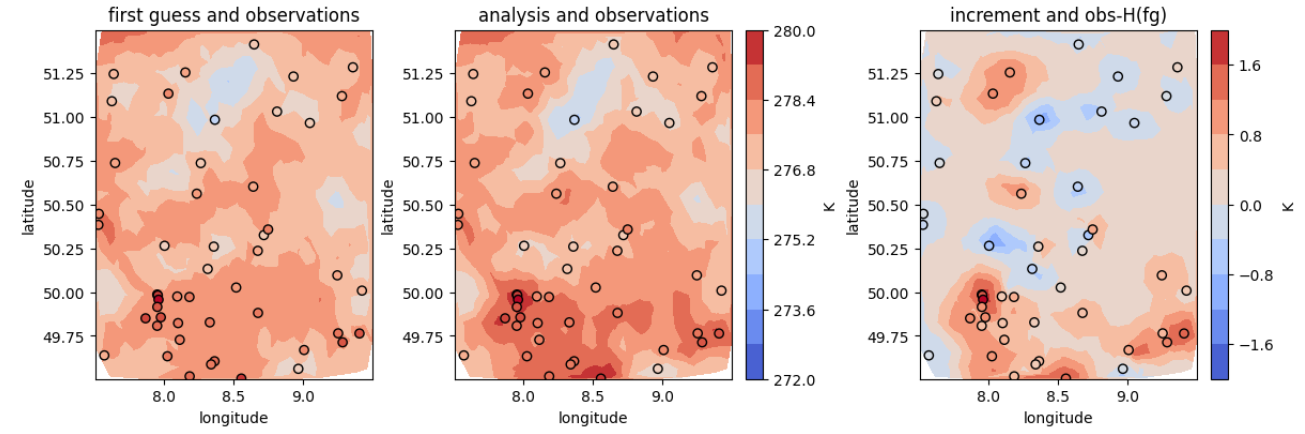
\includegraphics[width=\textwidth]{images/aivar5.png}
\caption{Comparison of AI-Var results with SYNOP observations. The left panel overlays observations on the first guess, the middle panel overlays them on the analysis, and the right panel shows the increment together with the observation minus background residuals. The increment pattern aligns with the differences between the forecast and observations.}
\end{figure}

%------------------------------------------------------------------------------
%
%------------------------------------------------------------------------------
\subsection{Plotting Fields and Observations}

In addition to statistical plots, we can plot the forecast, analysis, and increment fields. We also visualize the observations and compare them to the model output.

\begin{codeonly}{Plotting Fields and Observations}
fig, axs = plt.subplots(1,3, figsize = (12,4), constrained_layout=True)

time_step = "20230110000000"
vmin, vmax = 274., 280.

# plot forecast
plot_description = {
     "plot_type" : "fg",
     "time_step" : time_step,
     "plot_style" : "scatter",
     "layer_description" : ["T_2M", 2],
     "plot_settings" : {"cmap": "RdBu_r", "vmin": vmin, "vmax": vmax},
     "axis_settings" : {"title": "first guess", "xlabel": "longitude", "ylabel": "latitude"},
}
plotting.infer_plots(axs[0], inference, plot_description)

# plot analysis
plot_description["plot_type"] = "an"
plotting.infer_plots(axs[1], inference, plot_description)

# plot increment
plot_description["plot_type"] = "inc"
plotting.infer_plots(axs[2], inference, plot_description)
\end{codeonly}

These plots show the comparison between the forecast, analysis, and increment for the selected time step.

